\documentclass[../main.tex]{subfiles}
\begin{document}
\chapter{Array dan Matriks}

\section*{Tujuan Praktikum}
Setelah menyelesaikan praktikum ini, mahasiswa diharapkan mampu:
\begin{itemize}
  \item Memahami konsep array sebagai struktur data fundamental
  \item Mendeklarasikan, menginisialisasi, dan mengakses elemen array satu dimensi
  \item Melakukan operasi dasar pada array (pencarian, penjumlahan, maksimum/minimum)
  \item Memahami dan mengimplementasikan array dua dimensi untuk representasi matriks
  \item Melakukan operasi matriks (penjumlahan, perkalian, transpose)
  \item Memahami alokasi memori array dan perbedaan array statis vs dinamis
  \item Menerapkan best practices untuk keamanan akses array dan menghindari buffer overflow
\end{itemize}

\section{Pengantar Array}

\subsection{Konsep Dasar Array}
Array adalah struktur data fundamental yang menyimpan sekumpulan elemen bertipe sama secara kontigu (berurutan) di memori, memungkinkan akses cepat dengan kompleksitas \(O(1)\) menggunakan indeks. Array merupakan salah satu struktur data paling dasar dan penting dalam pemrograman untuk menyimpan koleksi data seperti daftar nilai, matriks, tabel, dan buffer \parencite{cpp-reference,free-pascal-docs,iso-c-draft-n1570,tutorialspoint-c-arrays}.

Keuntungan utama array adalah:
\begin{itemize}
  \item \textbf{Akses cepat:} Elemen dapat diakses langsung menggunakan indeks dengan waktu konstan \(O(1)\)
  \item \textbf{Efisiensi memori:} Penyimpanan kontigu mengoptimalkan cache locality dan performa
  \item \textbf{Sederhana:} Struktur yang mudah dipahami dan digunakan
  \item \textbf{Prediktabel:} Ukuran dan layout memori diketahui sejak kompilasi (untuk array statis)
\end{itemize}

\subsection{Karakteristik Array}
Representasi kontigu di memori memaksimalkan locality cache dan performa operasi berulang. Setiap bahasa pemrograman memiliki cara berbeda dalam mendeklarasikan dan mengelola array \parencite{pascal-tutorial-wikibooks,cpp-std-array,cplusplus-arrays,tambahpinter-array}:

\begin{itemize}
  \item \textbf{Pascal:} Menggunakan batas indeks eksplisit (misalnya \texttt{array[1..10]}), memberikan fleksibilitas dalam menentukan rentang indeks
  \item \textbf{C:} Menggunakan ukuran sebagai bagian dari tipe (misalnya \texttt{int arr[10]}), indeks selalu dimulai dari 0
  \item \textbf{C++:} Menyediakan array gaya C dan \texttt{std::array} untuk array ukuran tetap dengan keamanan tipe yang lebih baik dan metode tambahan
\end{itemize}

\subsection{Terminologi Penting}
\begin{itemize}
  \item \textbf{Elemen:} Nilai individual yang disimpan dalam array
  \item \textbf{Indeks:} Posisi numerik elemen dalam array (dimulai dari 0 di C/C++, dapat disesuaikan di Pascal)
  \item \textbf{Ukuran/Length:} Jumlah total elemen yang dapat disimpan dalam array
  \item \textbf{Bounds:} Batas bawah dan batas atas indeks yang valid
  \item \textbf{Subscript:} Istilah lain untuk indeks, digunakan untuk mengakses elemen
\end{itemize}

\section{Array Satu Dimensi}

Array satu dimensi adalah bentuk array paling sederhana, di mana elemen-elemen tersusun dalam satu baris linear. Dapat dibayangkan seperti daftar atau barisan data yang berurutan \parencite{tutorialspoint-c-arrays,galuhratna-array-c}.

\subsection{Deklarasi Array Satu Dimensi}
Deklarasi array mendefinisikan nama, tipe elemen, dan ukuran. Setiap bahasa memiliki sintaks berbeda namun konsep dasarnya sama \parencite{tutorialspoint-c-arrays,learncpp-arrays,free-pascal-docs,tutorialpemrograman-array-c}.

\textbf{Poin penting dalam deklarasi:}
\begin{itemize}
  \item Ukuran array harus diketahui pada waktu kompilasi (untuk array statis)
  \item Semua elemen harus bertipe data yang sama
  \item Memori dialokasikan secara kontigu untuk semua elemen
  \item Di C/C++, indeks dimulai dari 0, sehingga array berukuran $n$ memiliki indeks 0 sampai $n-1$
  \item Di Pascal, indeks dapat dimulai dari nilai apa pun yang ditentukan programmer
\end{itemize}

\textbf{Pascal:} Menggunakan sintaks \texttt{array[batas\_bawah..batas\_atas] of tipe}
\begin{lstlisting}[language=Pascal, caption={Deklarasi array di Pascal}]
var
  nilai: array[1..10] of integer;      // 10 integer, indeks 1-10
  huruf: array[0..25] of char;         // 26 karakter, indeks 0-25
  suhu: array[1..7] of real;           // 7 bilangan real
\end{lstlisting}

\textbf{C:} Menggunakan sintaks \texttt{tipe nama[ukuran]}. Indeks selalu dimulai dari 0.
\begin{lstlisting}[language=C, caption={Deklarasi array di C}]
int nilai[10];        // 10 integer, indeks 0-9
char huruf[26];       // 26 karakter, indeks 0-25
float suhu[7];        // 7 float
\end{lstlisting}

\textbf{C++:} Selain array gaya C, tersedia \texttt{std::array} yang lebih aman \parencite{cpp-std-array,cppreference-array}.
\begin{lstlisting}[language=C++, caption={Deklarasi array di C++}]
#include <array>

int nilai[10];                    // Array gaya C
std::array<int, 10> nilai2;       // std::array, lebih aman
std::array<char, 26> huruf;       // 26 karakter
std::array<double, 7> suhu;       // 7 double
\end{lstlisting}

\subsection{Inisialisasi dan Pengisian Array Satu Dimensi}
Array dapat diinisialisasi saat deklarasi atau diisi kemudian melalui loop atau akses langsung. Inisialisasi yang tepat penting untuk menghindari penggunaan nilai sampah (garbage value) yang tidak terduga \parencite{geeksforgeeks-array-init,learncpp-arrays,tambahpinter-array}.

\textbf{Metode pengisian array:}
\begin{itemize}
  \item \textbf{Inisialisasi langsung:} Memberikan nilai pada saat deklarasi
  \item \textbf{Pengisian individual:} Mengisi elemen satu per satu menggunakan indeks
  \item \textbf{Pengisian dengan loop:} Menggunakan struktur perulangan untuk mengisi seluruh atau sebagian array
  \item \textbf{Input dari pengguna:} Membaca nilai dari input keyboard
  \item \textbf{Nilai default:} Beberapa bahasa mengisi dengan nilai default (misalnya 0 untuk numerik)
\end{itemize}

\textbf{Pascal:} Inisialisasi manual atau dengan loop
\begin{lstlisting}[language=Pascal, caption={Inisialisasi array di Pascal}]
var
  nilai: array[1..5] of integer;
  i: integer;
begin
  // Pengisian langsung
  nilai[1] := 10;
  nilai[2] := 20;
  nilai[3] := 30;
  nilai[4] := 40;
  nilai[5] := 50;
  
  // Atau dengan loop
  for i := 1 to 5 do
    nilai[i] := i * 10;
end.
\end{lstlisting}

\textbf{C:} Mendukung inisialisasi dengan list initializer
\begin{lstlisting}[language=C, caption={Inisialisasi array di C}]
// Inisialisasi saat deklarasi
int nilai[5] = {10, 20, 30, 40, 50};
int angka[] = {1, 2, 3};  // ukuran otomatis: 3
int data[5] = {1, 2};     // sisanya diisi 0: {1, 2, 0, 0, 0}

// Pengisian dengan loop
int hasil[5];
for (int i = 0; i < 5; i++) {
  hasil[i] = i * 10;
}
\end{lstlisting}

\textbf{C++:} Seperti C, plus uniform initialization dan algoritme STL
\begin{lstlisting}[language=C++, caption={Inisialisasi array di C++}]
#include <array>
#include <algorithm>

// Inisialisasi gaya C
int nilai[5] = {10, 20, 30, 40, 50};

// std::array dengan uniform initialization
std::array<int, 5> angka = {1, 2, 3, 4, 5};
std::array<int, 5> data{};  // semua elemen diisi 0

// Menggunakan algoritme fill
std::array<int, 5> hasil;
std::fill(hasil.begin(), hasil.end(), 42);
\end{lstlisting}

\subsection{Menampilkan Output Array Satu Dimensi}
Untuk menampilkan isi array, gunakan loop untuk iterasi setiap elemen. Menampilkan array dengan format yang baik membantu dalam debugging dan presentasi hasil \parencite{tutorialspoint-c-arrays,cplusplus-arrays,galuhratna-array-c}.

\textbf{Teknik penampilan array:}
\begin{itemize}
  \item \textbf{Satu baris:} Menampilkan semua elemen dalam satu baris, dipisahkan spasi atau koma
  \item \textbf{Dengan indeks:} Menampilkan indeks dan nilai setiap elemen
  \item \textbf{Terformat:} Menggunakan lebar field tetap untuk alignment yang rapi
  \item \textbf{Range-based:} Di C++ modern, menggunakan range-based for loop yang lebih ringkas
\end{itemize}

\textbf{Pascal:}
\begin{lstlisting}[language=Pascal, caption={Menampilkan array di Pascal}]
var
  nilai: array[1..5] of integer = (10, 20, 30, 40, 50);
  i: integer;
begin
  // Tampilkan satu per satu
  for i := 1 to 5 do
    Write(nilai[i], ' ');
  Writeln;
  
  // Atau dengan High() untuk batas atas
  for i := Low(nilai) to High(nilai) do
    Writeln('nilai[', i, '] = ', nilai[i]);
end.
\end{lstlisting}

\textbf{C:}
\begin{lstlisting}[language=C, caption={Menampilkan array di C}]
#include <stdio.h>

int main() {
  int nilai[5] = {10, 20, 30, 40, 50};
  
  // Tampilkan dalam satu baris
  for (int i = 0; i < 5; i++) {
    printf("%d ", nilai[i]);
  }
  printf("\n");
  
  // Tampilkan dengan indeks
  for (int i = 0; i < 5; i++) {
    printf("nilai[%d] = %d\n", i, nilai[i]);
  }
  return 0;
}
\end{lstlisting}

\textbf{C++:}
\begin{lstlisting}[language=C++, caption={Menampilkan array di C++}]
#include <iostream>
#include <array>

int main() {
  std::array<int, 5> nilai = {10, 20, 30, 40, 50};
  
  // Dengan loop tradisional
  for (size_t i = 0; i < nilai.size(); i++) {
    std::cout << nilai[i] << " ";
  }
  std::cout << "\n";
  
  // Dengan range-based for (C++11)
  for (int n : nilai) {
    std::cout << n << " ";
  }
  std::cout << "\n";
  
  return 0;
}
\end{lstlisting}

\subsection{Operasi Dasar pada Array Satu Dimensi}
Operasi umum meliputi iterasi, pencarian, transformasi, dan validasi. Pada C++ pertimbangkan algoritme standar untuk menggantikan loop manual \parencite{cppreference-algorithm,gnu-c-manual}.

\begin{lstlisting}[language=Pascal, caption={Operasi dasar array di Pascal}]
var
  a: array[1..5] of integer;
  i, jumlah, maks: integer;
begin
  // Isi array
  for i := 1 to 5 do
    a[i] := i * i;
    
  // Hitung jumlah
  jumlah := 0;
  for i := 1 to 5 do
    jumlah := jumlah + a[i];
    
  // Cari maksimum
  maks := a[1];
  for i := 2 to 5 do
    if a[i] > maks then
      maks := a[i];
      
  Writeln('Jumlah: ', jumlah);
  Writeln('Maksimum: ', maks);
end.
\end{lstlisting}

\begin{lstlisting}[language=C, caption={Operasi dasar array di C}]
#include <stdio.h>

void fill(int *p, int n) {
  for (int i = 0; i < n; ++i)
    p[i] = i * i;
}

int main() {
int a[5];
fill(a, 5);  // a terdegradasi menjadi int*
  
  // Hitung jumlah
  int jumlah = 0;
  for (int i = 0; i < 5; i++)
    jumlah += a[i];
    
  printf("Jumlah: %d\n", jumlah);
  return 0;
}
\end{lstlisting}

\begin{lstlisting}[language=C++, caption={Operasi dengan std::array dan algoritme}]
#include <array>
#include <algorithm>
#include <numeric>
#include <iostream>

int main() {
  std::array<int, 5> a{};
  
  // Generate nilai
  int v = 1;
  std::generate(a.begin(), a.end(), [&]{ return v * v++; });
  
  // Hitung jumlah
  int jumlah = std::accumulate(a.begin(), a.end(), 0);
  
  // Cari maksimum
  auto maks = *std::max_element(a.begin(), a.end());
  
  std::cout << "Jumlah: " << jumlah << "\n";
  std::cout << "Maksimum: " << maks << "\n";
  std::cout << "Elemen terakhir: " << a.back() << "\n";
  
  return 0;
}
\end{lstlisting}

Validasi batas sebelum akses merupakan kebiasaan penting, terutama ketika indeks berasal dari input pengguna. Uji unit untuk indeks pertama dan terakhir membantu mencegah kesalahan off-by-one.

\subsection{Penyalinan dan Perbandingan Array (C/C++)}
Array di C tidak dapat ditugaskan langsung antar-variabel (akan terdegradasi menjadi pointer pada parameter fungsi). Gunakan loop atau fungsi perpustakaan untuk menyalin/banding.

\begin{lstlisting}[language=C, caption={Salin dan bandingkan isi array (C)}]
#include <string.h> // memcpy, memcmp

int a[5] = {1,2,3,4,5};
int b[5];
memcpy(b, a, sizeof a);     // salin bitwise
int sama = memcmp(a, b, sizeof a) == 0; // bandingkan
\end{lstlisting}

\begin{lstlisting}[language=C++, caption={Salin/cek kesetaraan (C++)}]
#include <array>
#include <algorithm>

std::array<int,5> a{1,2,3,4,5}, b{};
std::copy(a.begin(), a.end(), b.begin());
bool sama = (a == b); // std::array mendukung perbandingan leksikografis
\end{lstlisting}

\subsection{Contoh Program Lengkap: Pengolahan Data Nilai}

Berikut adalah contoh program lengkap yang mendemonstrasikan deklarasi, pengisian, dan operasi pada array satu dimensi untuk mengelola data nilai mahasiswa.

\textbf{Pascal:} Program pengolahan nilai mahasiswa
\begin{lstlisting}[language=Pascal, caption={Program lengkap array 1D di Pascal}]
program PengolahanNilai;
var
  nilai: array[1..10] of real;
  jumlah, rata: real;
  maksimum, minimum: real;
  i, n: integer;
begin
  // Input jumlah data
  Write('Masukkan jumlah mahasiswa (max 10): ');
  Readln(n);
  
  // Input nilai
  Writeln('Masukkan nilai mahasiswa:');
  for i := 1 to n do
  begin
    Write('Nilai mahasiswa ke-', i, ': ');
    Readln(nilai[i]);
  end;
  
  // Hitung jumlah dan cari maksimum/minimum
  jumlah := 0;
  maksimum := nilai[1];
  minimum := nilai[1];
  for i := 1 to n do
  begin
    jumlah := jumlah + nilai[i];
    if nilai[i] > maksimum then
      maksimum := nilai[i];
    if nilai[i] < minimum then
      minimum := nilai[i];
  end;
  rata := jumlah / n;
  
  // Tampilkan hasil
  Writeln;
  Writeln('=== Hasil Analisis ===');
  Writeln('Jumlah total: ', jumlah:0:2);
  Writeln('Nilai rata-rata: ', rata:0:2);
  Writeln('Nilai tertinggi: ', maksimum:0:2);
  Writeln('Nilai terendah: ', minimum:0:2);
end.
\end{lstlisting}

\textbf{C:} Program pengolahan nilai mahasiswa
\begin{lstlisting}[language=C, caption={Program lengkap array 1D di C}]
#include <stdio.h>

int main() {
  float nilai[10];
  float jumlah, rata, maksimum, minimum;
  int i, n;
  
  // Input jumlah data
  printf("Masukkan jumlah mahasiswa (max 10): ");
  scanf("%d", &n);
  
  // Validasi input
  if (n < 1 || n > 10) {
    printf("Jumlah mahasiswa tidak valid!\n");
    return 1;
  }
  
  // Input nilai
  printf("Masukkan nilai mahasiswa:\n");
  for (i = 0; i < n; i++) {
    printf("Nilai mahasiswa ke-%d: ", i + 1);
    scanf("%f", &nilai[i]);
  }
  
  // Hitung jumlah dan cari maksimum/minimum
  jumlah = 0;
  maksimum = nilai[0];
  minimum = nilai[0];
  for (i = 0; i < n; i++) {
    jumlah += nilai[i];
    if (nilai[i] > maksimum)
      maksimum = nilai[i];
    if (nilai[i] < minimum)
      minimum = nilai[i];
  }
  rata = jumlah / n;
  
  // Tampilkan hasil
  printf("\n=== Hasil Analisis ===\n");
  printf("Jumlah total: %.2f\n", jumlah);
  printf("Nilai rata-rata: %.2f\n", rata);
  printf("Nilai tertinggi: %.2f\n", maksimum);
  printf("Nilai terendah: %.2f\n", minimum);
  
  return 0;
}
\end{lstlisting}

\textbf{C++:} Program dengan \texttt{std::array}
\begin{lstlisting}[language=C++, caption={Program lengkap array 1D di C++}]
#include <iostream>
#include <array>
#include <algorithm>
#include <numeric>
#include <iomanip>

int main() {
  std::array<double, 10> nilai;
  int n;
  
  // Input jumlah data
  std::cout << "Masukkan jumlah mahasiswa (max 10): ";
  std::cin >> n;
  
  // Validasi input
  if (n < 1 || n > 10) {
    std::cout << "Jumlah mahasiswa tidak valid!\n";
    return 1;
  }
  
  // Input nilai
  std::cout << "Masukkan nilai mahasiswa:\n";
  for (int i = 0; i < n; i++) {
    std::cout << "Nilai mahasiswa ke-" << (i + 1) << ": ";
    std::cin >> nilai[i];
  }
  
  // Hitung jumlah menggunakan std::accumulate
  double jumlah = std::accumulate(nilai.begin(), 
                                   nilai.begin() + n, 0.0);
  double rata = jumlah / n;
  
  // Cari maksimum dan minimum
  auto maks_ptr = std::max_element(nilai.begin(), 
                                    nilai.begin() + n);
  auto min_ptr = std::min_element(nilai.begin(), 
                                   nilai.begin() + n);
  
  // Tampilkan hasil
  std::cout << "\n=== Hasil Analisis ===\n";
  std::cout << std::fixed << std::setprecision(2);
  std::cout << "Jumlah total: " << jumlah << "\n";
  std::cout << "Nilai rata-rata: " << rata << "\n";
  std::cout << "Nilai tertinggi: " << *maks_ptr << "\n";
  std::cout << "Nilai terendah: " << *min_ptr << "\n";
  
  return 0;
}
\end{lstlisting}

\subsection{Best Practices dan Peringatan}

\textbf{Keamanan Akses Array:}
\begin{itemize}
  \item Selalu validasi indeks sebelum mengakses array untuk mencegah buffer overflow
  \item Di C/C++, akses di luar batas dapat menyebabkan \textit{undefined behavior} yang berbahaya
  \item Pascal Free Pascal biasanya melakukan bounds checking secara default
  \item Gunakan \texttt{std::array::at()} di C++ untuk akses dengan bounds checking otomatis
\end{itemize}

\textbf{Inisialisasi Array:}
\begin{itemize}
  \item Selalu inisialisasi array sebelum digunakan untuk menghindari nilai sampah
  \item Di C/C++, array lokal tidak diinisialisasi secara otomatis
  \item Gunakan \texttt{\{\}} di C++ untuk zero-initialization
  \item Pascal biasanya mengisi dengan nilai 0 untuk tipe numerik
\end{itemize}

\textbf{Kesalahan Umum:}
\begin{itemize}
  \item \textbf{Off-by-one error:} Melupakan bahwa array C/C++ dimulai dari indeks 0
  \item \textbf{Buffer overflow:} Menulis ke luar batas array
  \item \textbf{Ukuran salah:} Menggunakan ukuran yang salah dalam loop
  \item \textbf{Type mismatch:} Mencampur tipe data yang tidak compatible
  \item \textbf{Uninitialized:} Membaca array yang belum diinisialisasi
\end{itemize}

\section{Array Multidimensi (Dua Dimensi)}

Array multidimensi memperluas konsep array ke dua dimensi atau lebih untuk memodelkan struktur seperti matriks, tabel, grid, atau data tabular lainnya. Array dua dimensi dapat divisualisasikan sebagai tabel dengan baris dan kolom, di mana setiap elemen diakses menggunakan dua indeks \parencite{iso-c-draft-n1570,cpp-reference,tutorialspoint-2d-arrays,duniailkom-cpp-2d-array}.

\subsection{Konsep Array Dua Dimensi}

Array 2D pada dasarnya adalah "array dari array" --- sebuah array yang setiap elemennya adalah array lain. Ini sangat berguna untuk:
\begin{itemize}
  \item \textbf{Matriks matematika:} Operasi aljabar linear
  \item \textbf{Tabel data:} Menyimpan data tabular seperti spreadsheet
  \item \textbf{Grid dan peta:} Representasi ruang 2D dalam game dan simulasi
  \item \textbf{Gambar digital:} Pixel sebagai matriks nilai warna
  \item \textbf{Graf dan graf adjacency matrix:} Representasi hubungan antar node
\end{itemize}

\subsection{Layout Memori Array 2D}

Pascal dan C mendukung array bertingkat dengan layout \textbf{row-major} (elemen baris disimpan berturutan di memori). Dalam layout row-major, elemen \texttt{arr[0][0]}, \texttt{arr[0][1]}, \texttt{arr[0][2]} disimpan berurutan, diikuti oleh \texttt{arr[1][0]}, \texttt{arr[1][1]}, \texttt{arr[1][2]}, dan seterusnya \parencite{free-pascal-docs,cplusplus-multidimensional}.

Formula akses linear untuk array 2D berukuran \texttt{M×N}:
\[
\mathrm{indeks\_linear} = \mathrm{baris} \times N + \mathrm{kolom}
\]

\begin{figure}[H]
  \centering
  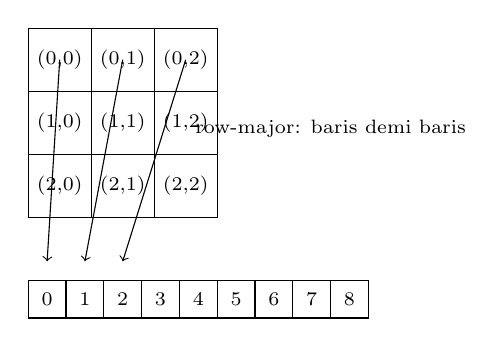
\begin{tikzpicture}[x=0.8cm,y=0.8cm]
    % Grid 3x3 dengan koordinat (baris, kolom)
    \foreach \i in {0,1,2} {
      \foreach \j in {0,1,2} {
        \draw (\j,-\i) rectangle +(1,-1);
        \node at (\j+0.5,-\i-0.5) {\scriptsize (\i,\j)};
      }
    }
    % Deretan indeks linear di bawah
    \foreach \k in {0,1,2,3,4,5,6,7,8} {
      \draw (\k*0.6,-4) rectangle +(0.6,-0.6);
      \node at (\k*0.6+0.3,-4.3) {\scriptsize \k};
    }
    % Panah dari baris pertama ke indeks linear 0..2
    \draw[->] (0.5,-0.5) -- (0.3,-3.7);
    \draw[->] (1.5,-0.5) -- (0.9,-3.7);
    \draw[->] (2.5,-0.5) -- (1.5,-3.7);
    \node at (4.8,-1.6) {\scriptsize row-major: baris demi baris};
  \end{tikzpicture}
  \caption{Pemetaan indeks 2D ke indeks linear (row-major)}
  \label{fig:row-major-mapping}
\end{figure}

\subsection{Representasi Datar (Flattened Buffer) dan Akses}
Pada representasi datar, elemen 2D disimpan dalam satu array 1D. Indeks liniernya \texttt{idx = baris * lebar + kolom}. Pendekatan ini mengurangi alokasi berulang dan meningkatkan locality memori.

\begin{lstlisting}[language=C, caption={Helper untuk indeks linier 2D pada buffer datar (C)}]
#include <stddef.h>

static inline size_t idx2d(size_t row, size_t col, size_t ncols) {
  return row * ncols + col;
}

// contoh akses
// int *buf = malloc(nrows * ncols * sizeof *buf);
// buf[idx2d(i, j, ncols)] = 42;
\end{lstlisting}

\begin{lstlisting}[language=C++, caption={Representasi datar dengan std::vector (C++)}]
#include <vector>
#include <stdexcept>

struct Matrix {
  size_t rows{}, cols{};
  std::vector<int> data; // ukuran = rows*cols
  Matrix(size_t r, size_t c): rows(r), cols(c), data(r*c) {}
  int& at(size_t r, size_t c) {
    if (r >= rows || c >= cols) throw std::out_of_range("idx");
    return data[r*cols + c];
  }
};
\end{lstlisting}

C++ dapat menggunakan array multidimensi built-in atau buffer datar dengan perhitungan indeks manual untuk kontrol performa yang lebih baik.

\subsection{Deklarasi Array Dua Dimensi}

\textbf{Pascal:} Gunakan sintaks \texttt{array[batas1..batas2, batas3..batas4] of tipe}
\begin{lstlisting}[language=Pascal, caption={Deklarasi array 2D di Pascal}]
var
  matriks: array[1..3, 1..4] of integer;    // 3 baris, 4 kolom
  tabel: array[0..2, 0..3] of real;         // 3x4 real
  grid: array[1..10, 1..10] of char;        // grid 10x10 karakter
\end{lstlisting}

\textbf{C:} Gunakan sintaks \texttt{tipe nama[baris][kolom]}
\begin{lstlisting}[language=C, caption={Deklarasi array 2D di C}]
int matriks[3][4];        // 3 baris, 4 kolom
float tabel[3][4];        // 3x4 float
char grid[10][10];        // grid 10x10 karakter
\end{lstlisting}

\textbf{C++:} Selain array gaya C, dapat menggunakan \texttt{std::array} bertingkat
\begin{lstlisting}[language=C++, caption={Deklarasi array 2D di C++}]
#include <array>

// Array gaya C
int matriks[3][4];

// std::array bertingkat (lebih aman)
std::array<std::array<int, 4>, 3> mat2;  // 3 baris, 4 kolom
std::array<std::array<double, 5>, 5> mat3;  // matriks 5x5
\end{lstlisting}

\subsection{Inisialisasi dan Pengisian Array Dua Dimensi}

Array dua dimensi dapat diinisialisasi dengan nested initializer atau diisi menggunakan nested loop. Pengisian array 2D memerlukan dua level iterasi: satu untuk baris dan satu untuk kolom \parencite{geeksforgeeks-2d-array,learncpp-multidimensional,duniailkom-cpp-2d-array}.

\textbf{Metode pengisian array 2D:}
\begin{itemize}
  \item \textbf{Nested initializer:} Inisialisasi langsung dengan kurung kurawal bertingkat
  \item \textbf{Nested loop:} Menggunakan dua loop bersarang (outer untuk baris, inner untuk kolom)
  \item \textbf{Input pengguna:} Membaca nilai baris per baris dari keyboard
  \item \textbf{Formula matematika:} Mengisi berdasarkan rumus (misalnya untuk matriks identitas)
  \item \textbf{Copy dari array lain:} Menyalin nilai dari array 2D yang sudah ada
\end{itemize}

\textbf{Pascal:} Pengisian dengan nested loop
\begin{lstlisting}[language=Pascal, caption={Inisialisasi array 2D di Pascal}]
var
  mat: array[1..3, 1..3] of integer;
  i, j: integer;
begin
  // Pengisian manual
  mat[1,1] := 1; mat[1,2] := 2; mat[1,3] := 3;
  mat[2,1] := 4; mat[2,2] := 5; mat[2,3] := 6;
  mat[3,1] := 7; mat[3,2] := 8; mat[3,3] := 9;
  
  // Atau dengan nested loop
  for i := 1 to 3 do
    for j := 1 to 3 do
      mat[i,j] := (i-1) * 3 + j;
end.
\end{lstlisting}

\textbf{C:} Inisialisasi dengan nested braces
\begin{lstlisting}[language=C, caption={Inisialisasi array 2D di C}]
// Inisialisasi saat deklarasi
int mat[3][3] = {
  {1, 2, 3},
  {4, 5, 6},
  {7, 8, 9}
};

// Atau tanpa nested braces (kurang jelas)
int mat2[2][3] = {1, 2, 3, 4, 5, 6};

// Pengisian dengan loop
int hasil[3][4];
for (int i = 0; i < 3; i++) {
  for (int j = 0; j < 4; j++) {
    hasil[i][j] = i * 4 + j;
  }
}
\end{lstlisting}

\textbf{C++:} Inisialisasi dengan uniform initialization
\begin{lstlisting}[language=C++, caption={Inisialisasi array 2D di C++}]
#include <array>
#include <algorithm>

// Array gaya C
int mat[3][3] = {
  {1, 2, 3},
  {4, 5, 6},
  {7, 8, 9}
};

// std::array dengan nested initialization
std::array<std::array<int, 3>, 3> mat2 = {{
  {1, 2, 3},
  {4, 5, 6},
  {7, 8, 9}
}};

// Inisialisasi semua elemen ke 0
std::array<std::array<int, 3>, 3> mat3{};

// Pengisian dengan nested loop
for (auto& baris : mat3) {
  std::fill(baris.begin(), baris.end(), 42);
}
\end{lstlisting}

\subsection{Menampilkan Output Array Dua Dimensi}

Untuk menampilkan array 2D, gunakan nested loop untuk iterasi baris dan kolom \parencite{cplusplus-multidimensional,tutorialspoint-2d-arrays}.

\textbf{Pascal:}
\begin{lstlisting}[language=Pascal, caption={Menampilkan array 2D di Pascal}]
var
  mat: array[1..3, 1..3] of integer;
  i, j: integer;
begin
  // Isi matriks
  for i := 1 to 3 do
    for j := 1 to 3 do
      mat[i,j] := (i-1) * 3 + j;
  
  // Tampilkan dalam format matriks
  Writeln('Matriks 3x3:');
  for i := 1 to 3 do begin
    for j := 1 to 3 do
      Write(mat[i,j]:4);  // format lebar 4
    Writeln;
  end;
end.
\end{lstlisting}

\textbf{C:}
\begin{lstlisting}[language=C, caption={Menampilkan array 2D di C}]
#include <stdio.h>

int main() {
  int mat[3][3] = {
    {1, 2, 3},
    {4, 5, 6},
    {7, 8, 9}
  };
  
  printf("Matriks 3x3:\n");
  for (int i = 0; i < 3; i++) {
    for (int j = 0; j < 3; j++) {
      printf("%4d", mat[i][j]);
    }
    printf("\n");
  }
  
  return 0;
}
\end{lstlisting}

\textbf{C++:}
\begin{lstlisting}[language=C++, caption={Menampilkan array 2D di C++}]
#include <iostream>
#include <array>
#include <iomanip>

int main() {
  std::array<std::array<int, 3>, 3> mat = {{
    {1, 2, 3},
    {4, 5, 6},
    {7, 8, 9}
  }};
  
  std::cout << "Matriks 3x3:\n";
  
  // Dengan nested loop tradisional
  for (size_t i = 0; i < mat.size(); i++) {
    for (size_t j = 0; j < mat[i].size(); j++) {
      std::cout << std::setw(4) << mat[i][j];
    }
    std::cout << "\n";
  }
  
  // Atau dengan range-based for
  std::cout << "\nDengan range-based for:\n";
  for (const auto& baris : mat) {
    for (int elemen : baris) {
      std::cout << std::setw(4) << elemen;
    }
    std::cout << "\n";
  }
  
  return 0;
}
\end{lstlisting}

\subsection{Operasi pada Array Dua Dimensi}

Operasi umum pada matriks: penjumlahan, perkalian, transpose, dan pencarian elemen \parencite{geeksforgeeks-matrix-operations}.

\begin{lstlisting}[language=Pascal, caption={Transpose matriks di Pascal}]
var
  mat, trans: array[1..3, 1..3] of integer;
  i, j: integer;
begin
  // Isi matriks
  for i := 1 to 3 do
    for j := 1 to 3 do
      mat[i,j] := (i-1) * 3 + j;
  
  // Transpose
  for i := 1 to 3 do
    for j := 1 to 3 do
      trans[j,i] := mat[i,j];
  
  // Tampilkan hasil
  Writeln('Matriks transpose:');
  for i := 1 to 3 do begin
    for j := 1 to 3 do
      Write(trans[i,j]:4);
    Writeln;
  end;
end.
\end{lstlisting}

\begin{lstlisting}[language=C, caption={Penjumlahan matriks di C}]
#include <stdio.h>

void tambah_matriks(int a[3][3], int b[3][3], int hasil[3][3]) {
  for (int i = 0; i < 3; i++)
    for (int j = 0; j < 3; j++)
      hasil[i][j] = a[i][j] + b[i][j];
}

int main() {
  int a[3][3] = {{1,2,3}, {4,5,6}, {7,8,9}};
  int b[3][3] = {{9,8,7}, {6,5,4}, {3,2,1}};
  int hasil[3][3];
  
  tambah_matriks(a, b, hasil);
  
  printf("Hasil penjumlahan:\n");
  for (int i = 0; i < 3; i++) {
    for (int j = 0; j < 3; j++)
      printf("%4d", hasil[i][j]);
    printf("\n");
  }
  
  return 0;
}
\end{lstlisting}

\begin{lstlisting}[language=C++, caption={Operasi matriks di C++}]
#include <iostream>
#include <array>

template<size_t N>
void transpose(const std::array<std::array<int, N>, N>& mat,
               std::array<std::array<int, N>, N>& trans) {
  for (size_t i = 0; i < N; i++)
    for (size_t j = 0; j < N; j++)
      trans[j][i] = mat[i][j];
}

int main() {
  std::array<std::array<int, 3>, 3> mat = {{
    {1, 2, 3},
    {4, 5, 6},
    {7, 8, 9}
  }};
  
  std::array<std::array<int, 3>, 3> trans;
  transpose(mat, trans);
  
  std::cout << "Matriks transpose:\n";
  for (const auto& baris : trans) {
    for (int elem : baris)
      std::cout << elem << " ";
    std::cout << "\n";
  }
  
  return 0;
}
\end{lstlisting}

Pada representasi datar, indeks linier dapat dihitung dengan rumus \texttt{indeks = baris * lebar + kolom}. Pendekatan ini mengurangi alokasi berulang dan meningkatkan locality memori, terutama untuk operasi numerik intensif. Sertakan fungsi pembantu untuk menerjemahkan koordinat ke indeks linier agar kesalahan penghitungan dapat diminimalkan.

\subsection{Contoh Program Lengkap: Operasi Matriks}

Berikut adalah contoh program lengkap yang mendemonstrasikan operasi matriks menggunakan array dua dimensi.

\textbf{Pascal:} Program penjumlahan dan perkalian matriks
\begin{lstlisting}[language=Pascal, caption={Program operasi matriks di Pascal}]
program OperasiMatriks;
const
  MAKS = 10;
var
  A, B, Hasil: array[1..MAKS, 1..MAKS] of integer;
  baris, kolom, i, j, k: integer;
  pilihan: integer;

procedure InputMatriks(var M: array of integer; 
                       br, kl: integer; nama: string);
var i, j: integer;
begin
  Writeln('Input matriks ', nama, ' (', br, 'x', kl, '):');
  for i := 1 to br do
    for j := 1 to kl do
    begin
      Write('Elemen [', i, ',', j, ']: ');
      Readln(M[i, j]);
    end;
end;

procedure TampilMatriks(M: array of integer; 
                        br, kl: integer; nama: string);
var i, j: integer;
begin
  Writeln('Matriks ', nama, ':');
  for i := 1 to br do
  begin
    for j := 1 to kl do
      Write(M[i, j]:4);
    Writeln;
  end;
  Writeln;
end;

procedure JumlahMatriks(A, B: array of integer;
                        var Hasil: array of integer;
                        br, kl: integer);
var i, j: integer;
begin
  for i := 1 to br do
    for j := 1 to kl do
      Hasil[i, j] := A[i, j] + B[i, j];
end;

begin
  Write('Masukkan jumlah baris: ');
  Readln(baris);
  Write('Masukkan jumlah kolom: ');
  Readln(kolom);
  
  if (baris > MAKS) or (kolom > MAKS) then
  begin
    Writeln('Ukuran terlalu besar! Maksimum ', MAKS, 'x', MAKS);
    Exit;
  end;
  
  // Input dua matriks
  InputMatriks(A, baris, kolom, 'A');
  Writeln;
  InputMatriks(B, baris, kolom, 'B');
  Writeln;
  
  // Penjumlahan
  JumlahMatriks(A, B, Hasil, baris, kolom);
  
  // Tampilkan hasil
  TampilMatriks(A, baris, kolom, 'A');
  TampilMatriks(B, baris, kolom, 'B');
  TampilMatriks(Hasil, baris, kolom, 'A + B');
end.
\end{lstlisting}

\textbf{C:} Program operasi matriks dengan fungsi
\begin{lstlisting}[language=C, caption={Program operasi matriks di C}]
#include <stdio.h>
#define MAKS 10

void input_matriks(int mat[][MAKS], int br, int kl, 
                   char nama) {
  printf("Input matriks %c (%dx%d):\n", nama, br, kl);
  for (int i = 0; i < br; i++) {
    for (int j = 0; j < kl; j++) {
      printf("Elemen [%d][%d]: ", i, j);
      scanf("%d", &mat[i][j]);
    }
  }
  printf("\n");
}

void tampil_matriks(int mat[][MAKS], int br, int kl, 
                    char nama) {
  printf("Matriks %c:\n", nama);
  for (int i = 0; i < br; i++) {
    for (int j = 0; j < kl; j++) {
      printf("%4d", mat[i][j]);
    }
    printf("\n");
  }
  printf("\n");
}

void jumlah_matriks(int A[][MAKS], int B[][MAKS],
                    int hasil[][MAKS], int br, int kl) {
  for (int i = 0; i < br; i++)
    for (int j = 0; j < kl; j++)
      hasil[i][j] = A[i][j] + B[i][j];
}

void kali_matriks(int A[][MAKS], int B[][MAKS],
                  int hasil[][MAKS], 
                  int br_a, int kl_a, int kl_b) {
  // Inisialisasi hasil dengan 0
  for (int i = 0; i < br_a; i++)
    for (int j = 0; j < kl_b; j++)
      hasil[i][j] = 0;
  
  // Perkalian matriks
  for (int i = 0; i < br_a; i++)
    for (int j = 0; j < kl_b; j++)
      for (int k = 0; k < kl_a; k++)
        hasil[i][j] += A[i][k] * B[k][j];
}

int main() {
  int A[MAKS][MAKS], B[MAKS][MAKS], Hasil[MAKS][MAKS];
  int baris, kolom;
  
  printf("Masukkan jumlah baris: ");
  scanf("%d", &baris);
  printf("Masukkan jumlah kolom: ");
  scanf("%d", &kolom);
  
  if (baris > MAKS || kolom > MAKS) {
    printf("Ukuran terlalu besar!\n");
    return 1;
  }
  
  // Input matriks
  input_matriks(A, baris, kolom, 'A');
  input_matriks(B, baris, kolom, 'B');
  
  // Penjumlahan
  jumlah_matriks(A, B, Hasil, baris, kolom);
  
  // Tampilkan hasil
  tampil_matriks(A, baris, kolom, 'A');
  tampil_matriks(B, baris, kolom, 'B');
  tampil_matriks(Hasil, baris, kolom, 'C');
  printf("C = A + B\n");
  
  return 0;
}
\end{lstlisting}

\textbf{C++:} Program dengan \texttt{std::array} dan template
\begin{lstlisting}[language=C++, caption={Program operasi matriks di C++}]
#include <iostream>
#include <array>
#include <iomanip>

template<size_t N, size_t M>
void inputMatriks(std::array<std::array<int, M>, N>& mat,
                  char nama) {
  std::cout << "Input matriks " << nama 
            << " (" << N << "x" << M << "):\n";
  for (size_t i = 0; i < N; i++) {
    for (size_t j = 0; j < M; j++) {
      std::cout << "Elemen [" << i << "][" << j << "]: ";
      std::cin >> mat[i][j];
    }
  }
  std::cout << "\n";
}

template<size_t N, size_t M>
void tampilMatriks(
    const std::array<std::array<int, M>, N>& mat,
    char nama) {
  std::cout << "Matriks " << nama << ":\n";
  for (const auto& baris : mat) {
    for (int elem : baris) {
      std::cout << std::setw(4) << elem;
    }
    std::cout << "\n";
  }
  std::cout << "\n";
}

template<size_t N, size_t M>
auto jumlahMatriks(
    const std::array<std::array<int, M>, N>& A,
    const std::array<std::array<int, M>, N>& B) {
  std::array<std::array<int, M>, N> hasil;
  for (size_t i = 0; i < N; i++)
    for (size_t j = 0; j < M; j++)
      hasil[i][j] = A[i][j] + B[i][j];
  return hasil;
}

template<size_t N, size_t M>
auto transposeMatriks(
    const std::array<std::array<int, M>, N>& mat) {
  std::array<std::array<int, N>, M> hasil;
  for (size_t i = 0; i < N; i++)
    for (size_t j = 0; j < M; j++)
      hasil[j][i] = mat[i][j];
  return hasil;
}

int main() {
  constexpr size_t BARIS = 3;
  constexpr size_t KOLOM = 3;
  
  std::array<std::array<int, KOLOM>, BARIS> A, B;
  
  // Input matriks
  inputMatriks(A, 'A');
  inputMatriks(B, 'B');
  
  // Operasi penjumlahan
  auto C = jumlahMatriks(A, B);
  
  // Operasi transpose
  auto AT = transposeMatriks(A);
  
  // Tampilkan hasil
  tampilMatriks(A, 'A');
  tampilMatriks(B, 'B');
  tampilMatriks(C, 'C');
  std::cout << "C = A + B\n\n";
  
  tampilMatriks(AT, 'A');
  std::cout << "A^T (Transpose A)\n";
  
  return 0;
}
\end{lstlisting}

\subsection{Aplikasi Praktis Array 2D}

\textbf{1. Sistem Penyimpanan Data Tabular}
\begin{lstlisting}[language=C, caption={Tabel data penjualan}]
// Penjualan 4 produk dalam 7 hari
int penjualan[7][4];  // [hari][produk]

// Hitung total penjualan per produk
for (int produk = 0; produk < 4; produk++) {
  int total = 0;
  for (int hari = 0; hari < 7; hari++) {
    total += penjualan[hari][produk];
  }
  printf("Total produk %d: %d\n", produk + 1, total);
}
\end{lstlisting}

\textbf{2. Representasi Grid/Papan Permainan}
\begin{lstlisting}[language=C++, caption={Papan catur 8x8}]
std::array<std::array<char, 8>, 8> papan;

// Inisialisasi papan kosong
for (auto& baris : papan)
  for (auto& sel : baris)
    sel = '.';

// Set posisi awal
papan[0][0] = 'R';  // Rook (Benteng) hitam
papan[0][4] = 'K';  // King (Raja) hitam
\end{lstlisting}

\textbf{3. Pengolahan Citra Sederhana}
\begin{lstlisting}[language=C, caption={Matriks pixel grayscale}]
#define LEBAR 640
#define TINGGI 480
unsigned char gambar[TINGGI][LEBAR];

// Inversi warna (negative)
for (int i = 0; i < TINGGI; i++)
  for (int j = 0; j < LEBAR; j++)
    gambar[i][j] = 255 - gambar[i][j];
\end{lstlisting}

\section{Alokasi Dinamis pada Array}
Ketika ukuran tidak diketahui di awal, gunakan alokasi dinamis. Di C, fungsi \texttt{malloc}, \texttt{free}, \texttt{realloc}; di C++ gunakan operator \texttt{new}/\texttt{delete} untuk alokasi manual; pada Pascal modern, array dinamis didukung \parencite{iso-c-draft-n1570,cpp-reference,free-pascal-docs,pascal-dynarray}.

\subsection{Contoh Dinamis}
\begin{lstlisting}[language=C, caption={malloc/realloc/free di C}]
#include <stdlib.h>

int *a = malloc(n * sizeof *a);
// ... isi a ...
int *tmp = realloc(a, m * sizeof *a);
if (tmp)
  a = tmp;
free(a);
\end{lstlisting}

\begin{lstlisting}[language=C++, caption={Alokasi dinamis array di C++}]
#include <iostream>
using namespace std;

int main() {
  int kapasitas = 100;
  int* arr = new int[kapasitas];
  int ukuran = 0;
  
  // Isi array
  for (int i = 0; i < 50; ++i) {
    arr[ukuran++] = i;
  }
  
  cout << "Ukuran: " << ukuran << ", Kapasitas: " << kapasitas << "\n";
  
  // Jangan lupa bebaskan memori
  delete[] arr;
}
\end{lstlisting}

\begin{lstlisting}[language=Pascal, caption={Array dinamis di Free Pascal}]
var
  a: array of integer;
  i: integer;
begin
  SetLength(a, 10);
  for i := 0 to High(a) do
    a[i] := i;
  SetLength(a, 20);
end.
\end{lstlisting}

Pastikan invarian kepemilikan memori dipertahankan pada semua jalur eksekusi, termasuk cabang kesalahan. Pada C++, gunakan RAII untuk memastikan pembebasan sumber daya meskipun terjadi pengecualian. Hindari penyalinan yang tidak perlu dengan menerapkan strategi \emph{move} dan peminjaman referensi yang jelas.

\section{Rangkuman}

Array merupakan struktur data fundamental yang sangat penting dalam pemrograman. Bab ini telah membahas konsep array dari dasar hingga aplikasi praktisnya.

\subsection{Poin-Poin Penting}

\textbf{Array Satu Dimensi:}
\begin{itemize}
  \item Array menyimpan sekumpulan elemen bertipe sama secara kontigu di memori
  \item Akses elemen menggunakan indeks dengan kompleksitas \(O(1)\)
  \item Di C/C++, indeks dimulai dari 0; di Pascal dapat disesuaikan
  \item Ukuran array statis harus diketahui saat kompilasi
  \item Selalu lakukan validasi bounds untuk menghindari buffer overflow
  \item Inisialisasi array sebelum digunakan untuk menghindari nilai sampah
\end{itemize}

\textbf{Array Dua Dimensi:}
\begin{itemize}
  \item Array 2D adalah "array dari array" yang merepresentasikan struktur tabel/matriks
  \item Akses elemen menggunakan dua indeks: baris dan kolom
  \item Layout memori menggunakan row-major order (baris berurutan)
  \item Cocok untuk matriks matematika, tabel data, grid, dan gambar digital
  \item Operasi umum: penjumlahan, perkalian, transpose matriks
  \item Gunakan nested loop untuk iterasi seluruh elemen
\end{itemize}

\textbf{Best Practices:}
\begin{itemize}
  \item Gunakan konstanta atau variabel untuk ukuran array, bukan magic numbers
  \item Validasi input dan batas indeks sebelum akses
  \item Pisahkan logika dengan fungsi untuk modularitas dan reusability
  \item Di C++, pertimbangkan \texttt{std::array} untuk type safety dan metode tambahan
  \item Dokumentasikan asumsi tentang ukuran dan batas array
  \item Gunakan nama variabel yang deskriptif untuk indeks (bukan hanya \texttt{i, j})
\end{itemize}

\section{Rangkuman Materi}
\begin{itemize}
  \item Array 1D/2D: deklarasi, inisialisasi, iterasi, dan operasi umum.
  \item Row-major memory layout dan pemetaan 2D\(\to\)1D (dengan diagram); helper indeks untuk buffer datar.
  \item Penyalinan/perbandingan array di C/C++; penggunaan algoritme STL pada C++.
  \item Kompleksitas waktu umum pada operasi array dan praktik validasi batas.
  \item Aplikasi praktis pada matriks, grid, citra, serta alokasi dinamis lintas bahasa.
\end{itemize}

\subsection{Perbandingan Array di Berbagai Bahasa}

\begin{table}[h]
\centering
\begin{tabular}{|l|c|c|c|}
\hline
\textbf{Fitur} & \textbf{Pascal} & \textbf{C} & \textbf{C++} \\
\hline
Indeks mulai & Fleksibel & 0 & 0 \\
\hline
Bounds checking & Ya (default) & Tidak & Tidak (kecuali \texttt{at()}) \\
\hline
Ukuran fleksibel & Array dinamis & Harus konstan & Array atau \texttt{std::array} \\
\hline
Sintaks deklarasi & \texttt{array[1..10]} & \texttt{int arr[10]} & \texttt{std::array<int,10>} \\
\hline
Keamanan tipe & Kuat & Lemah & Kuat (dengan \texttt{std::array}) \\
\hline
Inisialisasi & Manual/loop & List initializer & Uniform initialization \\
\hline
\end{tabular}
\caption{Perbandingan fitur array di Pascal, C, dan C++}
\end{table}

\subsection{Kapan Menggunakan Array}

\textbf{Gunakan Array ketika:}
\begin{itemize}
  \item Ukuran koleksi data diketahui dan tetap
  \item Perlu akses random dengan performa \(O(1)\)
  \item Memerlukan locality cache yang baik untuk performa
  \item Mengolah data numerik (vektor, matriks)
  \item Mengimplementasikan struktur data lain (stack, queue, heap)
\end{itemize}

\textbf{Pertimbangkan alternatif (linked list, vector) ketika:}
\begin{itemize}
  \item Ukuran tidak diketahui atau sering berubah
  \item Sering melakukan insert/delete di tengah koleksi
  \item Perlu fleksibilitas ukuran dinamis
  \item Ukuran sangat besar dan tidak semua elemen digunakan
\end{itemize}

\subsection{Kompleksitas Umum Operasi pada Array}
\begin{table}[H]
  \centering
  \caption{Kompleksitas waktu (asumsi array berukuran $n$)}
  \begin{tabular}{@{}lll@{}}
    \toprule
    Operasi & 1D & 2D (ukuran $n\\times n$) \\
    \midrule
    Akses indeks & $O(1)$ & $O(1)$ \\
    Pencarian linear & $O(n)$ & $O(n^2)$ \\
    Penyalinan penuh & $O(n)$ & $O(n^2)$ \\
    Penjumlahan elemen & $O(n)$ & $O(n^2)$ \\
    \bottomrule
  \end{tabular}
\end{table}

\subsection{Latihan Lanjutan}

Untuk memperdalam pemahaman tentang array, coba implementasikan:
\begin{enumerate}
  \item \textbf{Pencarian:} Linear search dan binary search pada array terurut
  \item \textbf{Sorting:} Bubble sort, selection sort, insertion sort
  \item \textbf{Rotasi array:} Geser elemen array ke kiri atau kanan
  \item \textbf{Merge array:} Gabungkan dua array terurut menjadi satu
  \item \textbf{Matriks sparse:} Representasi efisien matriks dengan banyak nilai 0
  \item \textbf{Operasi matriks:} Determinan, invers, perkalian Strassen
  \item \textbf{Game sederhana:} Tic-tac-toe, Sudoku solver, Conway's Game of Life
\end{enumerate}

Array adalah fondasi untuk memahami struktur data yang lebih kompleks. Penguasaan array yang baik akan memudahkan pembelajaran konsep-konsep pemrograman lanjutan seperti pointer, dynamic memory allocation, dan struktur data kompleks lainnya.

\end{document}
